\section{Computational complexity}
Let us define some notation.
\begin{defn}[Big $\mathbb{O}$ notation]
   Let $f$ be a real or complex valued function and $g$ a real valued function. Let both functions be defined on some unbounded subset of positive real numbers. One writes
   \begin{equation*}
       f(x) = \mathbb{O}(g(x)) \quad \text{as} \quad x \rightarrow a
   \end{equation*}
   if 
   \begin{equation*}
      \lim_{x \to a} \sup{\frac{\abs{f(x)}}{g(x)}} < \infty.
   \end{equation*}
   \end{defn}
   \begin{defn}[Big $\Omega$ Knuth notation]
      Let $f$ be a real or complex valued function and $g$ a real valued function. Let both functions be defined on some unbounded subset of positive real numbers. One writes
   \begin{equation*}
       f(x) = \Omega(g(x))
    \Longleftrightarrow
      g(x) = \mathbb{O}(f(x)).
   \end{equation*}
   \end{defn}
   

\subsection{Performance}\label{sec:performance}
Following the geometric interpretation of section~\ref{sec:geometric-interpretation} we are going to calculate the number of iterations $R$ necessary for the algorithm to find the solution. Each iteration rotates the state in the plane determined by $\ket{\psi}$ and $\ket{\beta}$, after $R$ iterations, the state is rotated by $\frac{2R + 1}{2}\theta$ from the $\ket{\alpha}$ axis. To optimize the probability of finding the solutions when we perform the measurement we will iterate until this angle is close to $\frac{\pi}{2}$, or
\begin{equation*}
    \frac{2R + 1}{2}\theta \simeq \frac{\pi}{2} \Rightarrow 2R + 1 \simeq \frac{\pi}{\theta},
\end{equation*}
we recall equation~\ref{eq:beta-projection} which we can approximate to
\begin{equation*}
    \theta \simeq 2\sqrt{\frac{M}{N}}
\end{equation*}
for $M<<N$ and large $N$. If we choose
\begin{equation*}
    R = \frac{\pi}{4}\sqrt{\frac{N}{M}} \biggl[1+\mathbb{O}\biggl(\frac{M}{N}\biggr)\biggr],
\end{equation*}
then the final probability of obtaining the measurement result $\ket{\beta}$ will be
\begin{equation*}
    \abs{\braket{\beta | \hat{G}^k | \psi}} = \sin^2\biggl(\frac{2R + 1}{2}\theta\biggr) = 1 - \mathbb{O}\biggl(\frac{M}{N}\biggl)
\end{equation*}
from which we can obtain an upper bound on the number of iterations required,
\begin{equation}\label{eq:upper-bound}
    R \leq \frac{\pi}{4} \sqrt{\frac{N}{M}}.
\end{equation}
That is, $R = \mathbb{O}\bigl(\sqrt{\frac{N}{M}}\bigr)$ iterations (and thus subroutine calls) must be performed in order to obtain a solution with a $\mathbb{O}\bigl(\frac{M}{N}\bigr)$ error; a quadratic improvement over the $\mathbb{O}\bigl(\frac{N}{M}\bigr)$ oracle calls required classically.

\subsubsection{An example with $M$ = 1 and $N$ = 4}
If we have $N = 4$ items and only a solution in the classical case an average of $\frac{N}{2} = 2$ subroutine calls would be needed to find the solution ($4$ in the worst case).
With the quantum search algorithm we have $\sin{\frac{\theta}{2}} = \sqrt{\frac{M}{N}} = \frac{1}{2}$ and thus $\frac{\theta}{2} = \frac{\pi}{6}$ and $\theta = \frac{\pi}{3}$. After one $\hat{G}$ iteration then, according to~\ref{eq:Gk}, we rotate $\ket{\psi}$ to a $\frac{\pi}{2}$ angle with $\ket{\alpha}$; that is, it lines up with $\ket{\beta}$.

When we measure by projecting onto the computational basis, we obtain the result $\ket{\beta}$ with certainty with just one iteration, a notable improvement over the classical case.

\subsection{Number of solutions}\label{sec:M}
Until now we assumed that $M\leq \frac{N}{2}$; if $M \geq \frac{N}{2}$ from the expression\footnote{We can demonstrate that $\sin\theta = 2\sqrt{\frac{M(N-M)}{N}}$.} $\theta=\arcsin\biggl(2\frac{\sqrt{M(N-M)}}{N}\biggr)$ we can see that $\theta$ get smaller as $M$ increase from $\frac{N}{2}$ to $N$. As a result the number of iterations needed by the search algorithm increases with $M$, for $M\geq \frac{N}{2}$.

We can distinguish two scenarios:
\begin{description}
   \item[$M$ is known] If $M$ is known \emph{a priori} to be larger than $\frac{N}{2}$ then we can just randomly pick an item from the search space and then check that it is a solution using the subroutine. This approach has a success probability at least one-half, and only requires one consultation with the oracle.
   \item[$M$ is not known] In the case where it isn't known whether $M\geq \frac{N}{2}$ we double the number of elements in the search space by adding $N$ extra items to it, none of which are solutions. We can do that adding a single qubit $\ket{x'}$ to the search index, doubling the number of items to be searched to $2N$. We then create a new augmented subroutine $\hat{U'}_\beta$ which marks an item only if it is a solution to the search problem and the extra bit is set to zero. The new search problem has then $M \leq 2N$ solutions and therefore running the algorithm with the subroutine $\hat{U'}_\beta$ at most $R$ calls to the subroutine are required, with $R$ as defined in~\ref{eq:upper-bound}; it follows that $\mathbb{O}\bigl(\frac{N}{M}\bigr)$ calls to $\hat{U}_\beta$ are required to perform the search.
   
\end{description}
\subsection{Optimality of the search algorithm}
It can be shown that no quantum algorithm can perform the task of searching through $N$ unsorted items using fewer than $\Omega(\sqrt{N})$ access to the subroutine\footnote{Again we restrict ourself in the case $M=1$.}, which means that
\begin{theorem}
The quantum search algorithm is asymptotically optimal. 
\end{theorem}
We take for granted some basic definitions of classical computational complexity theory and we proceed defying
\begin{defn}
\textbf{BPP} is the class of languages that can be solved in polynomial time by probabilistic Turing machines with error probability bounded by $1/3$. Using standard boosting techniques the error probability can then be made exponentially small in $k$ by iterating the algorithm $k$ times.
\end{defn}
\begin{defn}
\textbf{PSPACE} is the class of languages that may be solved on a Turing machine using a polynomial number of working bits, with no limitations on the amount of time that may be used by the machine.
\end{defn}
\begin{defn}
\textbf{BPQ} is the class of languages that can be solved in polynomial time by quantum Turing machines with error probability bounded by $1/3$. The error probability can be made exponentially small as in \textbf{BPP}.
\end{defn}
There are some evidence~\cite{Bennett_1997} that $\textbf{BQP} \neq \textbf{BPP}$ (i.e. polynomial-time quantum Turing machines are more powerful than polynomial-time probabilistic Turing machines). Since \textbf{BPP} is regarded as the class of all efficiently computable languages, this provides evidence that quantum computers could be inherently more powerful than classical computers in a model-independent way.

However exactly where \textbf{BQP} fits with respect to \textbf{P}, \textbf{NP} and \textbf{PSPACE} is as yet unknown. What is known is that quantum computers can solve all the problems in \textbf{P} efficiently and that there are no problems outside of \textbf{PSPACE} which they can solve efficiently. Therefore, \textbf{BQP} lies somewhere between \textbf{P} and \textbf{PSPACE}.
It has been demonstrated that
\begin{equation*}
   \textbf{P}   \subseteq \textbf{BPP} \subseteq \textbf{BQP}  \subseteq \textbf{PSPACE}
\end{equation*}
and so proving that $\textbf{BPP} \subset \textbf{BQP}$ would definitively establish that $\textbf{P} \subset \textbf{PSPACE}$, solving a major outstanding problem in computer science.
\begin{figure}[htb]
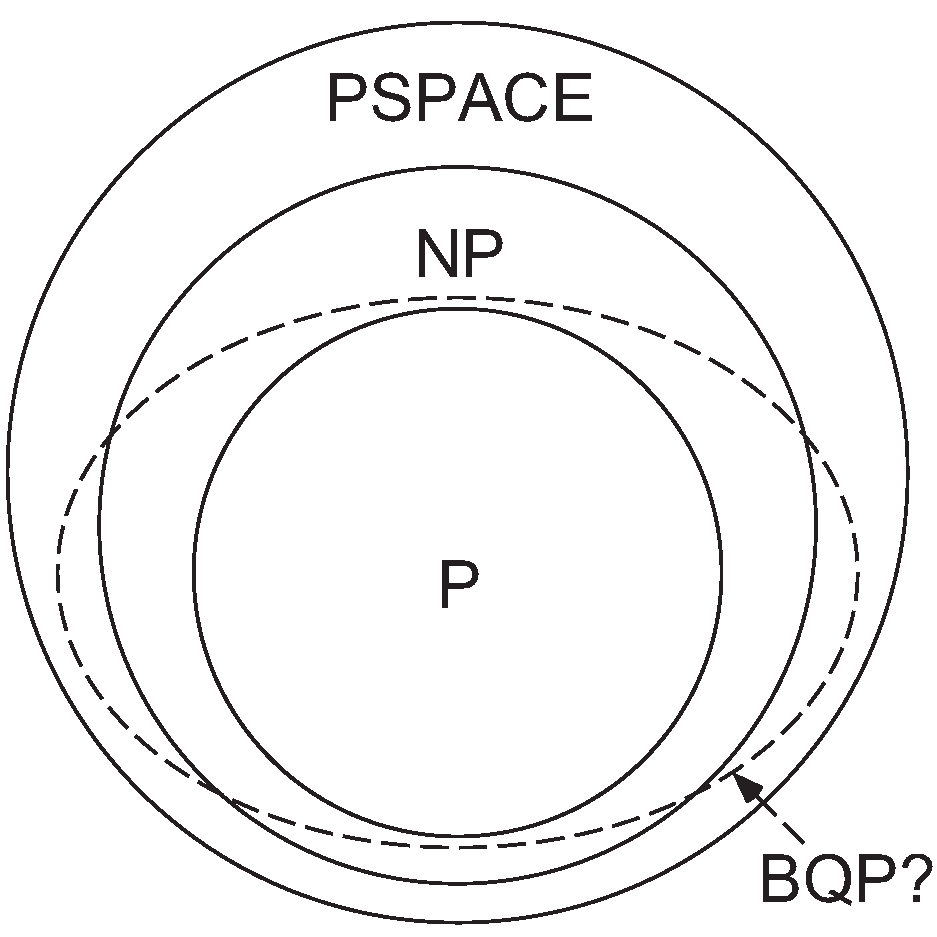
\includegraphics{computational-complexity.png}
\centering
\caption{The relationship between classical and quantum complexity classes.}
\end{figure}

Another open computational problem is $\textbf{NP} \stackrel{?}{\subseteq} \textbf{BQP}$.
We know that we can adopt the quantum search algorithm to solve any \textbf{NP}-complete\footnote{We can demonstrate that solving \textbf{NP}-complete problems in polynomial times would mean solving every other \textbf{NP} problem in polynomial time.} problem, with the subroutine checking all the proposed solutions to it.
The fact that the quantum search algorithm is optimal means that it is not possible to search an $N$ item search space using $\mathbb{O}(\log_2{N})$ calls of $\hat{U}_\beta$. If such an algorithm had existed, it would have allowed us to solve \textbf{NP}-complete problems efficiently on a quantum computer by transforming problems in \textbf{NP} into Grover-type search problems.

This does not rule out the possibility that \textbf{NP} $\subset$ \textbf{BQP}. What this result do establish is that there is no search-based method for attacking \textbf{NP}-complete problems.
However we note that it is widely believed that the search space of \textbf{NP}-complete problems has no structure and that the best possible method for solving such problems is to adopt an unstructured search method. Furthermore for many problems in the \textbf{NP}-complete class there is no better method known than exhaustive search of all the possible solution. If one takes this point of view this indicates that \textbf{BQP} does not contain \textbf{NP}-complete problems.

\subsection{Cryptography}
The quantum search algorithm can be seen as an algorithm for function inversion. If we have a function $y=f(x)$ that can be evaluated on a quantum computer, the quantum search algorithm allow us to calculate $x$ when given $y$.

Consequently, Grover's algorithm gives broad asymptotic speed-ups to many kinds of brute-force attacks on symmetric-key cryptography, including collision attacks\footnote{A collision attack on a cryptographic hash is a brute-force method that tries to find two inputs producing the same hash value.} and pre-image attacks\footnote{A pre-image attack on cryptographic hash functions is is a brute-force method that tries to find a message that has a specific hash value.}.
The algorithm could brute-force a $128$-bit symmetric cryptographic key in $R = \mathbb{O} \biggl(\sqrt{\frac{N}{M}}\biggr) = \mathbb{O} (\sqrt{N}) = \mathbb{O} (\sqrt{2^{128}}) = \mathbb{O} (2^{64})$ iterations and a 256-bit key (the actual standard for cryptography) in $\mathbb{O} (2^{128})$ iterations. Because of that  it is sometimes suggested~\cite{10.1007/978-3-642-12929-2_6} that symmetric key lengths be doubled to protect against future quantum attacks.
